\chapter{Quantum theory background}
\label{chpt:background}

%\addcontentsline{toc}{chapter}{\color{green}Background}

% can we have a quote by Feynman pls????
%\epigraph{\textit{No fair! You changed the outcome by measuring it!}}{Hubert Farnsworth}


\epigraph{I think I can safely say that nobody understands quantum mechanics}{\textit{Richard Feynman, The Character of Physical Law}}

\section{The Qubit}\label{TheBasics}

In this section we will introduce quantum mechanics and its basic unit of information, the qubit. In general a qubit is the name given to well defined two level systems that are governed by the laws of quantum physics. Any system that obeys the mathematical description of a qubit given in this chapter can in principle be used to perform quantum computation. The set of physical systems that fall into this category is diverse meaning there are many competing physical platforms being developed that are capable of quantum computation. The theory of quantum mechanics is mathematically described using linear algebra and so we advice that the reader should first review basic linear algebra concepts, such as basis vectors, matrices and tensor products, before continuing with this chapter.

In classical computing the fundamental unit of information is the familiar bit. Every bit is a binary number 0 or 1 that we use to represent false or true, or combine together to encode any information we wish. In quantum information theory, the fundamental unit of information is the qubit. The qubit, much like the bit, is a description of the state of a system. In the case of the bit, the system being described is a classical two level system, such as the transistor. This is also the case for the qubit, except now, the dynamics are dominated by quantum physics instead of classical physics, resulting in fundamentally different behaviour. To understand the differences in behaviour this brings about, we will first introduce the notions of quantum measurement and superposition.

Quantum mechanics is a measurement based theory in which we use our observations of a system to describe the state of that system in a mathematically precise way. In this regard, we describe the state of a qubit by measuring its value and noting down the outcome. This is the same as in the classical case expect now, the same state can give different measurement outcomes upon repeated measurement. As a result of this, the state description must capture the probabilistic nature of the measurement outcomes if it is to fully represent the qubit. Since the qubit is a two level system, the possible outcomes are binary valued '0' or '1', but crucially, if we prepare a qubit in the same state multiple times its value might not be consistent upon measurement. A qubit that gives non-consistent measurement outcomes is said to be in a \textit{superposition}.  Formally, we describe the qubit $\psi$ by its state $\ket{\psi}$. The notation $\ket{...}$ for the state of a system is standard in the field and was invented by one of the fore-fathers of Quantum physics, Paul Dirac. For a more in depth introduction to Dirac notation please see \autoref{chpt:advancedtopics} or \textit{p13} of \cite{nielsen_chuang_2010}.

Given a qubit, $\ket{\psi}$, that when measured always gives the outcome 0, we say that $\psi$ is in the basis state $\ket{0}$:\\

\begin{equation}
    \ket{\psi}=\ket{0}\equiv\begin{pmatrix}  1\\ 0 \end{pmatrix}
\end{equation}

This state is not in a superposition and will always give '0' upon measurement. The states $\ket{0}$ and $\ket{1}$ are known as basis state and are used in linear combinations to formally describe superposition state. This terminology comes from linear algebra in which basis vectors are used to represent arbitrary vectors in a vector space. In the same way, basis states are used to form arbitrary superposition states of a qubit. Given a second qubit $\ket{\phi}$, now in a superposition of basis states $\ket{0}$ and $\ket{1}$, we say that:

\begin{equation}\label{qubit}
    \ket{\phi}=\alpha\ket{0}+\beta\ket{1}\equiv\alpha \begin{pmatrix}  1\\ 0 \end{pmatrix} + \beta \begin{pmatrix} 0\\ 1 \end{pmatrix}
\end{equation}

The parameters $\alpha$ and $\beta$ preceding the basis state, known as amplitudes, are related to the probabilities of obtaining the corresponding values 0 or 1. More precisely, the probability of getting the state $\ket{0}$ is $\abs{\alpha}^{2}$ and the probability of getting the state $\ket{1}$ is $\abs{\beta}^{2}$. To continue drawing parallels with vector formalism, each basis state can be thought of as an orthonormal basis vector spanning the space of possible superpositions. Crucially, each basis state is independent of all others i.e. the inner product between $\ket{0}$ and $\ket{1}$ is 0.


In general, $\alpha$ and $\beta$ can take complex values and so to ensure that the probabilities are real we take the absolute value squared \cite{nielsen_chuang_2010} \textit{p80}. It is also the case that the probabilities sum to 1 since we must always get '0' or '1' upon measurement. The significance of having complex valued amplitudes is discussed briefly in \autoref{chpt:advancedtopics}. Taking the vector representation of both $\ket{\phi}$ and $\ket{1}$, then the probability of measuring $\ket{\phi}$ and obtaining the outcome 1, collapsing the superposition state $\ket{\phi}$ to the basis state $\ket{1}$, is given by the absolute value squared of their inner product.

In order to perform useful computations with qubits, we need to be able to control the state of a qubit. This is done by single qubit gates that take input states and map them to other input states. These gates are described further in (REF) but an example of a particularly important gate, known as the Hadamard gate, is given below.

A gate (or operator as they are sometimes called) can be expressed in matrix form whereby each column maps a basis state to a new combination. For example, take the Hadamard operator H that maps each basis sate $\ket{0}$ and $\ket{1}$ to equal superposition with opposite relative phase. This is a key operator is quantum computation because it maps basis states to superposition states. To represent $\hat{H}$ in matrix notation we write:

\begin{equation}
    \hat{H} = \frac{1}{\sqrt{2}}\begin{pmatrix}1 & 1\\
    1 & -1\end{pmatrix}
\end{equation}

The first column maps $\ket{0}$ to the state $\frac{1}{\sqrt{2}}(\ket{0}+\ket{1})\equiv\ket{+}$ and the second column maps $\ket{1}$ to $\frac{1}{\sqrt{2}}(\ket{0}-\ket{1})\equiv\ket{-}$. The states $\ket{+}$ and $\ket{-}$ are frequently used and so given their own names plus and minus. A gate can also be written in Dirac form in the following way:

\begin{equation}
    \hat{H}=\ket{+}\bra{0}+\ket{-}\bra{1}
\end{equation}

To see how this form is applied to a general state $\ket{\psi}$, see \autoref{chpt:advancedtopics}.

So far, our system is only capable of represent two unique points of information which we have assigned '0' and '1'. In practice, we need a system that has more than two basis states, giving us the facility to represent larger amounts of information. For this, we must generalise our description of a qubit to a multi-qubit system.


\section{Registers}


In order to encode large amounts of information into a system, the system must contain an orthonormal basis states for each information point. To access a larger space of basis states we can combine several qubits into so called registers, with each register going on to performing a specific task in a computation algorithm. Before we discuss how the capacity of a system scales with register size, let's introduce how to combine to qubits to form a 2-qubit register.

We combine qubits via the tensor product of each of the qubits individual basis states which combine to form a new set of basis states. This process enables us to build the basis states of the combined 2-qubit register one at a time. Let the state subscript denote qubits 1 (blue) and 2 (red) in the register, then the basis states of the combined register are given as follows:

\begin{equation}
\begin{split}
    \ket{\textcolor{blue}{0}}_1\otimes\ket{\textcolor{red}{0}}_2 \equiv\ket{\textcolor{blue}{0}\textcolor{red}{0}}\\
    \ket{\textcolor{blue}{0}}_1\otimes\ket{\textcolor{red}{1}}_2 \equiv\ket{\textcolor{blue}{0}\textcolor{red}{1}}\\
    \ket{\textcolor{blue}{1}}_1\otimes\ket{\textcolor{red}{0}}_2 \equiv\ket{\textcolor{blue}{1}\textcolor{red}{0}}\\
    \ket{\textcolor{blue}{1}}_1\otimes\ket{\textcolor{red}{1}}_2 \equiv\ket{\textcolor{blue}{1}\textcolor{red}{1}}
\end{split}
\end{equation}

We have conveniently chosen to labelled the four basis states with quantum numbers that give us information about the component basis states that form them. We can now assign 00 to 0, 01 to 1, 10 to 2 and 11 to 3 in a binary encoding of the integers 0-3. Note that sometimes in the literature, authors will write $\ket{0}\ket{1}$ instead of $\ket{01}$, however, they are equivalent.

Thus an arbitrary superposition state of the 2-qubit register can now take the form:

\begin{equation}
    \ket{\psi}=a_{00}\ket{00}+a_{01}\ket{01}+a_{10}\ket{10}+a_{11}\ket{11} = \sum_{i,j=0}^{1}a_{ij}\ket{ij}
\end{equation}

For example, if the two qubits are in the state $\ket{\psi}_1 = \ket{+}$ and $\ket{\psi}_2 = \ket{-}$, respectively, then there joint state is described by:

\begin{equation}\label{twoQubit}
    \begin{split}
        \ket{\psi}_1 \otimes \ket{\psi}_2 &= \big(\frac{1}{\sqrt{2}}(\ket{\textcolor{blue}{0}}+\ket{\textcolor{blue}{1}})\big)_1 \otimes \big(\frac{1}{\sqrt{2}}(\ket{\textcolor{red}{0}}-\ket{\textcolor{red}{1}})\big)_2\\
        &= \frac{1}{2}(\ket{\textcolor{blue}{0}\textcolor{red}{0}}-\ket{\textcolor{blue}{0}\textcolor{red}{1}}+\ket{\textcolor{blue}{1}\textcolor{red}{0}}-\ket{\textcolor{blue}{1}\textcolor{red}{1}})
    \end{split}
\end{equation}

From Equation \ref{twoQubit} above, we can read out the probabilities of finding qubits 1 and 2 in each basis state. For example the probability of measuring the register and finding qubit 1 in the state '0' and qubit 2 in the state '1' is the absolute value squared of the amplitude preceding the basis state $\ket{01}$, in this case $\abs{\frac{1}{2}}^2 = \frac{1}{4}$. In fact, the probability distribution across each of the basis states is constant and equal to $\frac{1}{4}$ because the 2-qubit register is in an equal superposition.

The tensor product generalises to any size register and the number of basis states scale by $O(2^n)$ where $n$ is the number of qubits within the register. The power of quantum computation is a direct result of this scaling, combined with the fact that we can prepare a system to be in an equal superposition of all basis states at the same time. For example, if we were to assign each basis state to a specific entry in a large database, then we could prepare a large quantum system to be in a superposition of all the basis states and then perform computations on all data entries simultaneously.

\section{Quantum Computation}

To perform arbitrary operation on multi-qubit systems, it's possible to show that all one requires is single qubit control and two qubit gates that can be strung together into a sequence of operations. Therefore, a computation is mapped onto an equivalent string of single and two qubit gates performed on a register of qubits. In general, quantum algorithms can be broken down into the following key steps:

\begin{enumerate}
    \item Determine the number of qubits required to represent the domain of your computation and assign each basis state to an information point.
    \item Input the all '0' basis state in which all qubits are in the state '0' and create an equal superposition across all basis states.
    \item Convert the computation into a string of gates that typically allows the evaluation of your computation on all basis states simultaneously or in a resource efficient manor i.e. with relatively few gates.
    \item The result of each basis state computation is then encoded into the amplitudes of the corresponding basis state in such a way that suppresses the amplitude of all wrong answers and enhances the amplitude of all the correct answers.
    \item The overall register is then measured giving the correct answer with high probability, due to its enhanced amplitude. 
\end{enumerate}

The following is an example of how to apply multiple gates to a system. Say we have a system of 2 qubits and we want to act with both $\hat{H}$ on qubit 2 and $\hat{H}$ on qubit 2. The total operator we act on the 2-qubit register will be given by: $\hat{H}\otimes\hat{H}$ where the Hadamard acts on each qubit. This operation will map the input state $\ket{00}$ to an equal superposition across the registers basis state (as is requires in step 2 above). The corresponding matrix for this operation is given by the tensor product of each single gate matrix: 

\begin{equation}
\hat{H}\otimes\hat{H}=\frac{1}{\sqrt{2}}
\begin{blockarray}{cc}
    \ket{\textcolor{blue}{0}}_1 & \ket{\textcolor{blue}{1}}_1 \\
    \begin{block}{(cc)}
        1 & 1\\
        1 & -1\\
    \end{block}
\end{blockarray}\otimes\frac{1}{\sqrt{2}}
\begin{blockarray}{cc}
    \ket{\textcolor{red}{0}}_2 & \ket{\textcolor{red}{1}}_2 \\
    \begin{block}{(cc)}
        1 & 1\\
        1 & -1\\
    \end{block}
\end{blockarray}=\frac{1}{\sqrt{2}}  
\begin{blockarray}{cccc}
    \ket{\textcolor{blue}{0}\textcolor{red}{0}} & \ket{\textcolor{blue}{0}\textcolor{red}{1}} & \ket{\textcolor{blue}{1}\textcolor{red}{0}} & \ket{\textcolor{blue}{1}\textcolor{red}{1}} \\
    \begin{block}{(cccc)}
        1 & 1 & 1 & 1\\
        1 & -1 & 1 & 1\\
        1 & 1 & -1 & -1\\
        1 & -1 & -1 & 1\\
    \end{block}
\end{blockarray}
\end{equation}

From the above we can see how each of the 2-qubit basis states will map under the operation $\ket{H}\otimes\ket{H}$ by looking at the corresponding column. For example, $(\hat{H}\otimes\hat{H})\ket{00}=\frac{1}{2}(\ket{00}+\ket{01}+\ket{10}+\ket{11})$.
This is exactly the state needed in many quantum algorithms and serves as a starting point for computation. The operation described above is the implement ion of two single qubit gates, one on each qubit within the register. In order to perform computation, 2-qubit gates is required whose operation on one qubit depends upon the value of the other. A key example of this is the CNOT gate which performs a controlled-NOT operation on the second qubit, controlled by the value of the first. The matrix representaion of the CNOT is as follows:

\begin{equation}\label{CNOT}
\hat{CNOT}=
\begin{blockarray}{cccc}
    \ket{\textcolor{blue}{0}\textcolor{red}{0}} & \ket{\textcolor{blue}{0}\textcolor{red}{1}} & \ket{\textcolor{blue}{1}\textcolor{red}{0}} & \ket{\textcolor{blue}{1}\textcolor{red}{1}} \\
    \begin{block}{(cccc)}
        1 & 0 & 0 & 0\\
        0 & 1 & 0 & 0\\
        0 & 0 & 0 & 1\\
        0 & 0 & 1 & 0\\
    \end{block}
\end{blockarray}
\end{equation}

Let's act the CNOT gate on our equal superposition state to see how each basis state in the equal superposition is mapped:

\begin{equation}
    \hat{CNOT}\Big(\frac{1}{2}(\ket{00}+\ket{01}+\ket{10}+\ket{11})\Big)=\frac{1}{2}(\ket{00}+\ket{01}+\ket{11}+\ket{10})
\end{equation}

We can see that the third basis state, $\ket{10}$, is mapped to $\ket{11}$ and conversely the fourth term, $\ket{11}$, is mapped to $\ket{10}$. Since the value of the first qubit is '1' in both these cases, a NOT is performed on the value of the second qubit. Coincidentally, this results in the state remaining the same, however, this would not have been the case if the amplitudes of each basis state had not been the equal. The CNOT is necessarily a reversible gate, as is required by quantum mechanics (see \autoref{chpt:advancedtopics}). A list of important gates, along with a description of the gate circuit model, is given in the following section.

\section{Quantum gates and Measurement}

introduce in text and table
Cnot coherent classical XOR non separable can't write as a tensor product.
Clifford + T gateset 

This section briefly reviews the gate model for circuit based quantum computing and discusses the similarities between  digital and quantum computers. The gate model is one of the most popular architectures for quantum computation at the moment. A number of companies such as, \textit{Intel \cite{intelqcomp} IBM \cite{ibmqweb}, Google \cite{googleqai} and Rigetti \cite{rigetti}} are all using the gate model approach for quantum computing. There are other architectures for quantum computing however we think that the gate model is the most similar to digital computers.

Both forms of computation follow the same structure, you start with bits (or qubits), operations are performed on the (qu)bits and then you measure the new values of the (qu)bits. We show an example in \autoref{fig:basicoperation}.

%%%% digital circuit
\begin{figure}[H] 
\centering
\begin{subfigure}[h]{0.4\textwidth}
\begin{align*}
\Qcircuit @C=0.5cm @R=0.7cm
{&\lstick{A} &\multigate{2}{Operation} & \\
&\lstick{B} &\ghost{Operation} & \\
&& &\qw &\lstick{Q} \\}
\end{align*}
\caption{Digital operation}
\label{fig:digitalcirc}
\end{subfigure}
~
%%%% Q circuit
\begin{subfigure}[H]{0.4\textwidth}
\begin{align*}
\Qcircuit @C=0.5cm @R=0.7cm
{&\lstick{A} &\multigate{2}{Operation} &\qw &\lstick{A} \\
&\lstick{B} &\ghost{Operation} &\qw &\lstick{B} \\
&\lstick{Q} &\ghost{Operation} &\qw &\lstick{Q} \\}
\end{align*}
\caption{Quantum operation}
\label{fig:quantumcirc}
\end{subfigure}
\caption{Digital and quantum logic circuits for implementing an arbitrary operation on bits $A, B$ returning value $Q$}
\label{fig:basicoperation}
\end{figure}

One of the main differences between the two figures is that in the quantum circuit the inputs $A \& B$ exist after the operation and the output $Q$ is present before the operation. This is a feature of quantum computing being reversible (unitary).  

One of the requirements for quantum computing to be universal is that we are able to perform any single qubit and a single two qubit gate. Most quantum algorithms make use of a Hadamard gate at the beginning of the computation. 


\begin{figure}[H]
    \begin{align*}
    \Qcircuit @C=0.5cm @R=0.7cm
    {&\lstick{0} &\gate{H} &\qw &\rstick{\frac{0+1}{\sqrt{2}}} \\ 
    &\lstick{A} &\qw &\qw &\rstick{A} }
    \end{align*}
    \caption{Hadamard gate acting on the top qubit and no gate performed on the bottom qubit}
    \label{fig:mylabel1}
\end{figure}


Multiple qubits gates are of the form, control-\textit{Operation}, one of the most popular two-qubit gates used is the Controlled-NOT. The control means use the value of the first qubit to decide whether or not to perform the operation on the target qubit. 


\begin{figure}[H]
    \begin{align*}
    \Qcircuit @C=0.5cm @R=0.7cm
    {&\lstick{0} &\gate{H} &\qw &\rstick{0 \text{  if  } A=0, \text{  ELSE  } \frac{0+1}{\sqrt{2}} \text{  if  } A=1 } \\ 
    &\lstick{A} &\ctrl{-1} &\qw &\rstick{A} }
    \end{align*}
    \caption{Hadamard gate acting on the top qubit and no gate performed on the bottom qubit}
    \label{fig:mylabel2}
\end{figure}


\begin{comment}
\subsubsection{Digital logic}

Every digital computing operation can be built up from NAND logic gates \cite{sheffer1913set}. We can call a NAND logic gate a universal gate for computation. The NOR gate is also universal in the same way any computation can be constructed from NOR gates.

\begin{figure}[H]
  \centering
    \begin{subfigure}[h]{0.4\textwidth}
  \centering
  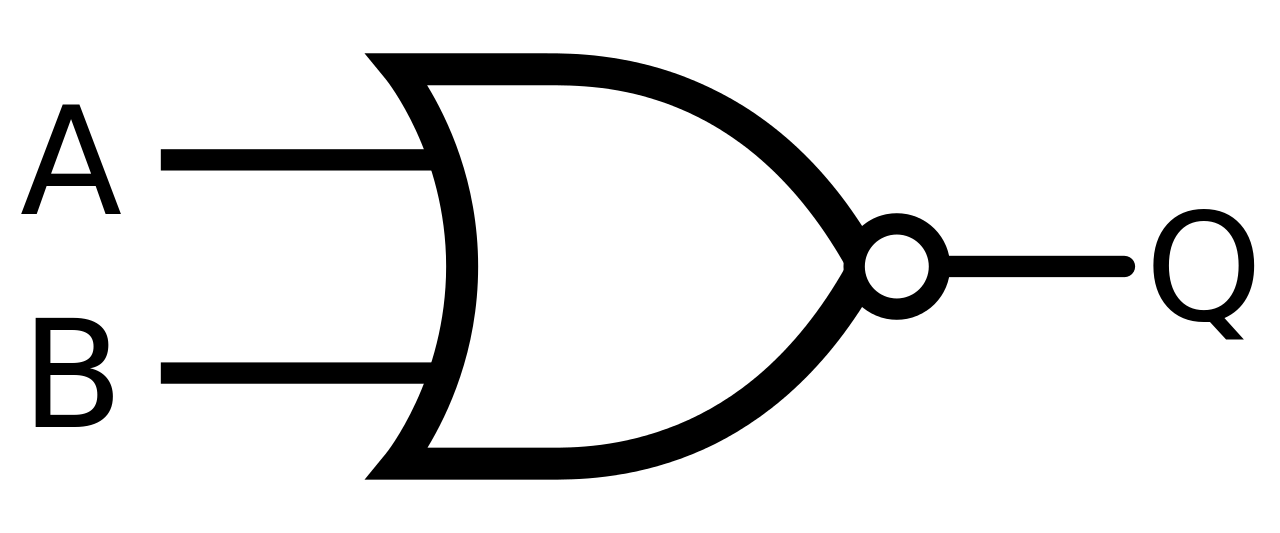
\includegraphics[width=0.7\textwidth]{NOR_ANSI_Labelled_svg.png}
  \caption{The NOR logic gate \cite{norwiki}.}
  \label{fig:NOR}
  \end{subfigure}
  ~
  \begin{subfigure}[h]{0.4\textwidth}
  \centering
  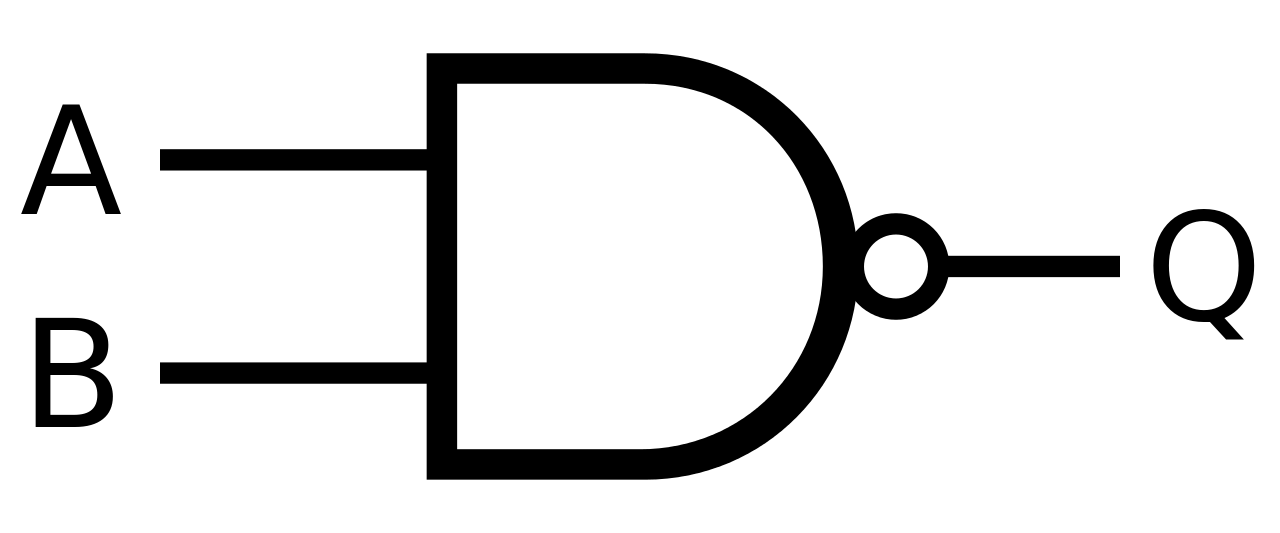
\includegraphics[width=0.7\textwidth]{NAND_ANSI_Labelled_svg.png}
  \caption{The NAND logic gate \cite{nandwiki}.}
  \label{fig:NAND}
\end{subfigure}
\end{figure}

\begin{table}[!htb]
    \caption{Global caption}
    \begin{subtable}{.5\linewidth}
      \centeringhttps://v2.overleaf.com/project/5b03e9ad40127f7bf2eb6ed5
        \begin{tabular}{|l|l||l|}
        \hline
        Input A & Input B & Output Q \\ \hline
        0       & 0       & 1       \\ 
        0       & 1       & 0       \\ 
        1       & 0       & 0       \\ 
        1       & 1       & 0       \\
        \hline
    \end{tabular}
    \caption{NOR gate truth table}
    \end{subtable}
    %
    \begin{subtable}{.5\linewidth}
      \centering
        \begin{tabular}{|l|l||l|}
        \hline
        Input A & Input B & Output Q \\ \hline
        0       & 0       & 1       \\ 
        0       & 1       & 1       \\ 
        1       & 0       & 1       \\ 
        1       & 1       & 0       \\
        \hline
    \end{tabular}
    \caption{NAND gate truth table}
    \end{subtable} 
\end{table}
\end{comment}

\newpage
\section{Gate cheat sheet}

\begin{comment}
We now list some of the common gates mentioned throughout the rest of this guide, the Clifford plus T gates.
\end{comment}

\begin{table}[h]
    \centering
    \begin{tabular}{c|c|c|c}
        Gate & Description &  Matrix representation & Dirac notation \\ \hline
        %
        $\boxed{X}$ & Bit flip 
        & $\begin{bmatrix} 0 & 1 \\ 1 & 0 \end{bmatrix}$ 
        & $\ket{0}\bra{1} + \ket{1}\bra{0}$\\
        %
        $\boxed{Z}$ & Phase flip 
        & $\begin{bmatrix} 1 & 0 \\ 0 &-1 \end{bmatrix}$ 
        & $\ket{0}\bra{0} - \ket{1}\bra{1} $\\
        %
        $\boxed{T}$ & Phase gate 
        & $\begin{bmatrix} 1 & 0 \\ 0 & \exp{i\pi/8} \end{bmatrix}$ 
        & $\ket{0}\bra{0} + \exp{i\pi / 8 }*\ket{1}\bra{1} $\\
        %
        $\boxed{H}$ & Superposition 
        & $\frac{1}{\sqrt{2}} \begin{bmatrix} 1 & 1 \\ 1&-1 \end{bmatrix}$ 
        & $\ket{0}\bra{0} + \ket{0}\bra{1} + \ket{1}\bra{0} - \ket{1}\bra{1} $\\ 
    \end{tabular}
    \caption{Single qubit gates}
    \label{tab:singlequbitgates}
\end{table}

\begin{table}[h]
    \centering
    \begin{tabular}{c|c|c|c}
        Gate & Description &  Matrix representation & Dirac notation \\ \hline
        %
        $\boxed{R_X(\theta)}$ & Rotation around the X axis 
        & $\begin{bmatrix} cos(\theta/2) & -isin(\theta/2) \\ -isin(\theta/2) & cos(\theta/2) \end{bmatrix}$ 
        & No.\\
        %
        $\boxed{R_Z(\theta)}$ & Rotation around the Z axis 
        & $\begin{bmatrix} \exp{i\theta/2} & 0 \\ 0 & \exp{-i\theta/2} \end{bmatrix}$ 
        & $\exp{i\theta/2}\ket{0}\bra{0} + \exp{-i\theta/2}\ket{1}\bra{1} $\\
    \end{tabular}
    \caption{Single qubit arbitrary rotation gates}
    \label{tab:singlequbitrotationgates}
\end{table}
\vspace{-10pt}
\begin{table}[h]
    \centering
    \begin{tabular}{c|c|c|c}
        Gate & Description &  Matrix representation & Dirac notation \\ \hline
        $\boxed{CNOT}$ or
        $\Qcircuit @C=0.5cm @R=0.7cm
        {&\targ &\qw\\ 
        &\ctrl{-1} &\qw}$
        & Controlled Bit flip & $\begin{bmatrix} 1 & 0 & 0 & 0 \\ 0 & 1 & 0 & 0 \\ 0 & 0 & 0 & 1 \\ 0 & 0 & 1 & 0 \end{bmatrix}$ 
        & $\ket{00}\bra{00} + \ket{01}\bra{01} + \ket{01}\bra{10} + \ket{10}\bra{11} $ \\
        %
        $\boxed{CPHASE}$ or
        $\Qcircuit @C=0.5cm @R=0.7cm
        {&\gate{Z} &\qw\\ 
        &\ctrl{-1} &\qw}$
        & Controlled Phase flip & $\begin{bmatrix} 1 & 0 & 0 & 0 \\ 0 & 1 & 0 & 0 \\ 0 & 0 & 1 & 0 \\ 0 & 0 & 0 & -1 \end{bmatrix}$ 
        & $\ket{00}\bra{00} + \ket{01}\bra{01} + &\ket{10}\bra{10} - \ket{11}\bra{11} $ \\
        %
        $\boxed{SWAP}$ or
        $\Qcircuit @C=0.5cm @R=0.7cm
        {&\qswap &\qw \\
        &\qswap \qwx &\qw}$
        & Swap qubits & $\begin{bmatrix} 1 & 0 & 0 & 0 \\ 0 & 0 & 1 & 0 \\ 0 & 1 & 0 & 0 \\ 0 & 0 & 0 & 1\end{bmatrix}$
        & $ \ket{00}\bra{00} + \ket{01}\bra{10} + \ket{10}\bra{01} + \ket{11}\bra{11} $
    \end{tabular}
    \caption{Two qubit (control) gates}
    \label{tab:twoqubitgates}
\end{table}


